\chapter{Applying IR2Vec to Thread Coarsening}
\label{chap:ch2}


\section{Introduction to IR2Vec}
% \subsection{Overview}
\vk{Should say what is IR2Vec here}
The overview of the proposed methodology is shown in Fig.~\ref{fig:IR2Vec-Overview}. Instructions in IR can be represented as an Entity-Relationship Graph, with the instruction entities as nodes, and the relation between the entities as edges. A translational learning model is used to learn these relations. The output of this learning is a dictionary containing the embeddings of the entities and is called \textit{Seed embedding vocabulary}. 

\begin{figure}[t]
    \centering
    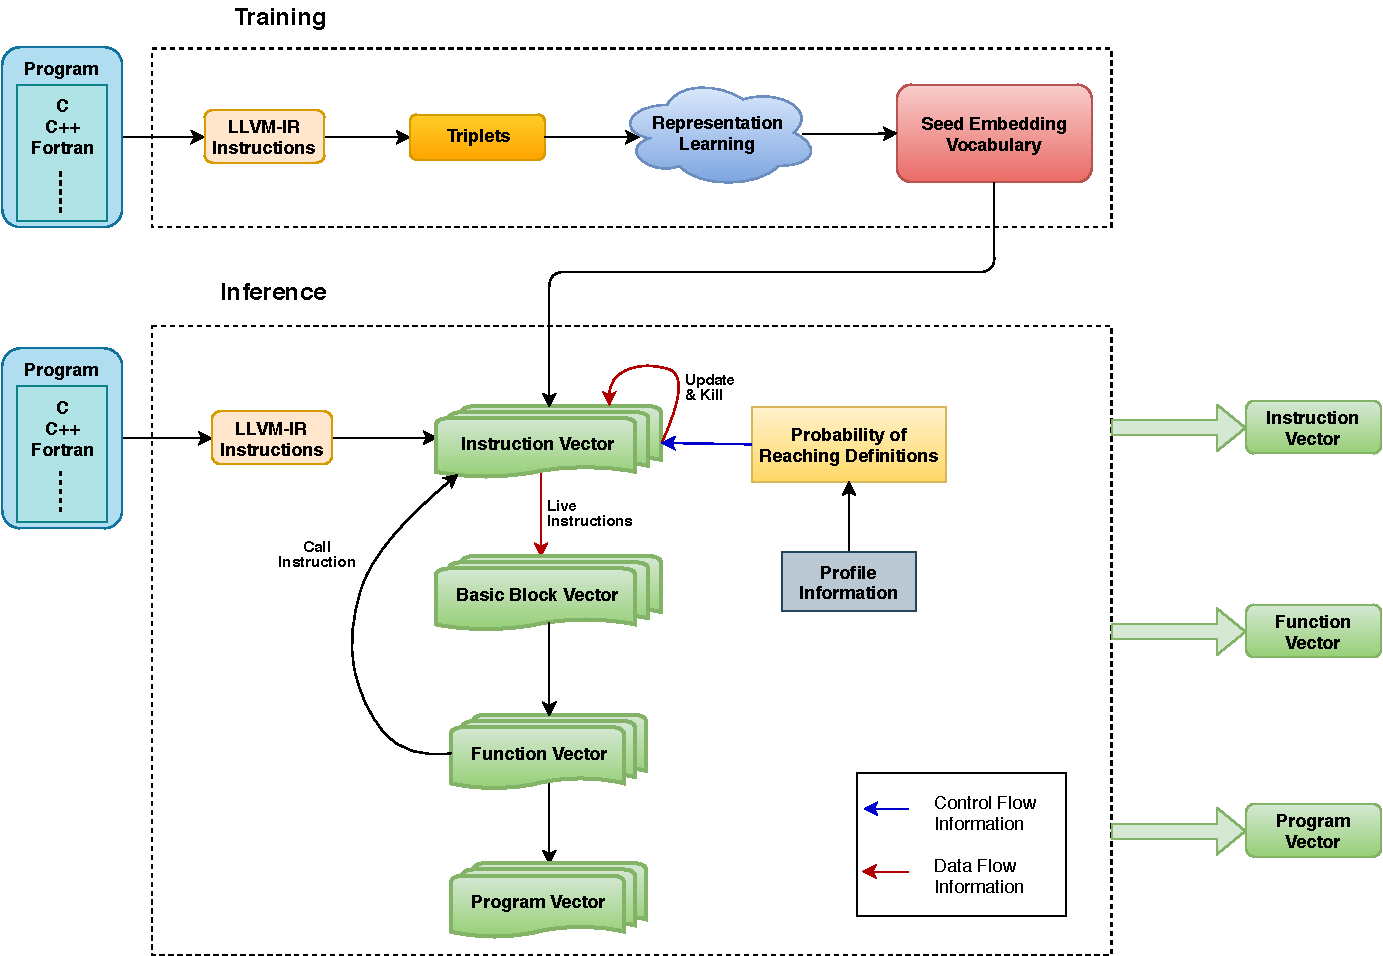
\includegraphics[scale=0.5]{figures/chapter-2/flow.pdf}
    \caption{Overview of IR2Vec infrastructure}
     \label{fig:IR2Vec-Overview}
\end{figure}

The above dictionary is looked up to form the embeddings at various levels of the input program. 
At the coarsest level, instruction embeddings are obtained just by using the \textit{Seed embedding vocabulary}. We call such encodings as \textit{Symbolic} encodings.
We use the \textit{Use-Def} and \textit{Reaching definition}~\cite{Hecht:1977:FAC:540175, muchnick1997advanced} information to form the instruction vector for \textit{Flow-Aware} encodings. 

The instructions which are \textit{live} are used to form the \textit{Basic block Vector}  using the flow analysis information. The vector to represent a function is obtained by using the basic block vectors of the function. The \textit{Code vector} is obtained by propagating the vectors obtained at the function level with the \texttt{call graph} information.
\section{Thread Coarsening Task}
Thread coarsening~\cite{Volkov-Demmel-10.5555/1413370.1413402} is the process of increasing the work done by a single thread by fusing two or more concurrent threads. Thread coarsening factor corresponds to the number of threads that can be fused together. Selection of an optimal thread coarsening factor can lead to significant improvements~\cite{Magni-SC13-DBLP:conf/sc/MagniDO13} in the speedups on GPU devices and a naive coarsening would lead to a substantial slowdown.

A thread coarsening factor of a kernel that gives the best speedup on a GPU could give the worst performance with the same coarsening factor on another device (either within or across vendors) because of the architectural characteristics of the device~\cite{magni2014automatic, Stawinoga-10.1145/3194242}. For example, \texttt{nbody} kernel, which has a higher degree of Instruction Level Parallelism, can be better exploited by VLIW based AMD Radeon than SIMD based AMD Tahiti~\cite{magni2014automatic}.

\subsection{Dataset} 
In this experiment, we follow the experimental setup proposed by Magni et al.~\cite{magni2014automatic} to predict the optimal thread coarsening factor---among $\{1,2,4,8,16,32\}$---for a given kernel specific to a GPU device. Even for this experiment, we use the dataset provided by Ben-Nun et al.~\cite{ncc}. It consists of about 68 datapoints from 17 OpenCL kernels on 4 different GPUs -- AMD Radeon 5900, AMD Tahiti 7970, NVIDIA GTX 480 and NVIDIA Tesla K20c.
These kernels are collectively taken from AMD SDK, NVIDIA SDK and Parboil benchmarks.
A datapoint consists of the kernel and its runtime corresponding to each thread coarsening factor on a particular GPU device.

\subsection{Experimental Setup}
Even for this task, we use gradient boosting classifier instead of LSTMs and RNNs to predict the coarsening factor for the four GPU targets. For this experiment, we set the learning rate as 0.05 with 140 decision stumps with 1 level, as the number of data points in the dataset is very low. We use ten-fold cross-validation for measuring the performance.

\begin{table}[h]
\centering
  \caption{\% improvement in speedup obtained by Flow-Aware encodings when compared to the other methods}
%   \vspace*{-\baselineskip}
  \label{tab:predictionSpeedup-tc}    \small
  \begin{tabular}{p{2.5cm}p{1.9cm}p{1.6cm}p{1.5cm}p{2.2cm}p{1.5cm}}
    \hline
    \textbf{Architecture} & \textbf{Magni et al. \cite{o2013portable-grewe}} & \textbf{DeepTune \cite{cummins2017end2end}} & \textbf{DeepTune-TL \cite{cummins2017end2end}} & \textbf{inst2vec \cite{ncc}}\footnotemark  & \textbf{IR2Vec  Symbolic}\\
    \hline
    \textbf{AMD Radeon 5900} & 27.66\% & 5.26\% & 5.26\% & 4.35\% & -- \\
    \textbf{AMD Tahiti 7970} & 25.41\% & 29.37\% & 36.56\% & 18.17\% & 2.08\% \\
    \textbf{NVIDIA GTX 480} & 45.31\% & 25.21\% & 18.89\% & 23.89\% & 3.98\%\\
    \textbf{NVIDIA Tesla K20c} & 52.84\% & 15.41\% & 11.98\% & 11.98\% & 0.18\%\\
\hline
\end{tabular}
\end{table}
\footnotetext{As per the results given in the NCC paper~\cite{ncc}, inst2vec-imm achieves a (arithmetic) mean of $ 1.28\times$, $ 1.18\times$, $ 1.11\times$ and $1\times$ speedup on AMD Radeon, AMD Tahiti, NVIDIA GTX and NVIDIA Tesla; whereas our \textit{Flow-Aware} encodings achieve a (arithmetic) mean of $ 1.25\times$, $ 1.3\times$, $ 1.26\times$ and $ 1.16\times$ respectively.}

\subsubsection{Speedups}
In Fig.~\ref{fig:tcSpeedup}, we show the speedups achieved by our encodings and earlier works on four different platforms -- AMD Radeon HD 5900, AMD Tahiti 7970, NVIDIA GTX 480 and NVIDIA Tesla K20c. 

On AMD Radeon, both of our encodings achieve a speedup of $ 1.2\times$ when compared to the state-of-the-art speedup of $ 1.15\times$ and $ 1.14\times$ achieved by inst2vec~\cite{ncc} and DeepTune model with transfer learning (DeepTune-TL)~\cite{cummins2017end2end}.
In AMD Tahiti, \textit{Flow-Aware} encodings achieve a speedup of $ 1.23\times$; \textit{Symbolic} encoding achieves a speedup of $ 1.2\times$, whereas the earlier works by DeepTune-TL and inst2vec achieve a speedup of $ 0.9\times$ and $ 1.04\times$ respectively. In Tab.~\ref{tab:predictionSpeedup-tc}, we show the percentage improvement of speedup obtained by \textit{Flow-Aware} encodings over other methodologies. From the table, we can infer that \textit{Flow-Aware} gives better results for every architecture when compared to the other methods. 

% \begin{figure}
%     \centering
%     \begin{tabular}{@{}c@{}}
%         \includegraphics[scale=0.55, width=\textwidth]{figures/TC/radeon.pdf}
%     \end{tabular}
%     % \vspace{-5cm}
%     \begin{tabular}{@{}c@{}}
%         \includegraphics[scale=0.55, width=\textwidth]{figures/TC/tahiti.pdf}
%     \end{tabular}
%     \begin{tabular}{@{}c@{}}
%         \includegraphics[scale=0.55, width=\textwidth]{figures/TC/gtx.pdf}
%     \end{tabular}
%     \begin{tabular}{@{}c@{}}
%         \includegraphics[scale=0.55, width=\textwidth]{figures/TC/tesla.pdf}
%     \end{tabular}
%     \caption{Plot showing the speedups achieved by predicted coarsening factors by various methods}
%     % \vspace*{-\baselineskip}
%     \label{fig:tcSpeedup}
%      \vspace*{-0.4cm}
% \end{figure}

% \begin{figure}
%     \centering
%     \begin{tabular}{@{}c@{}}
%         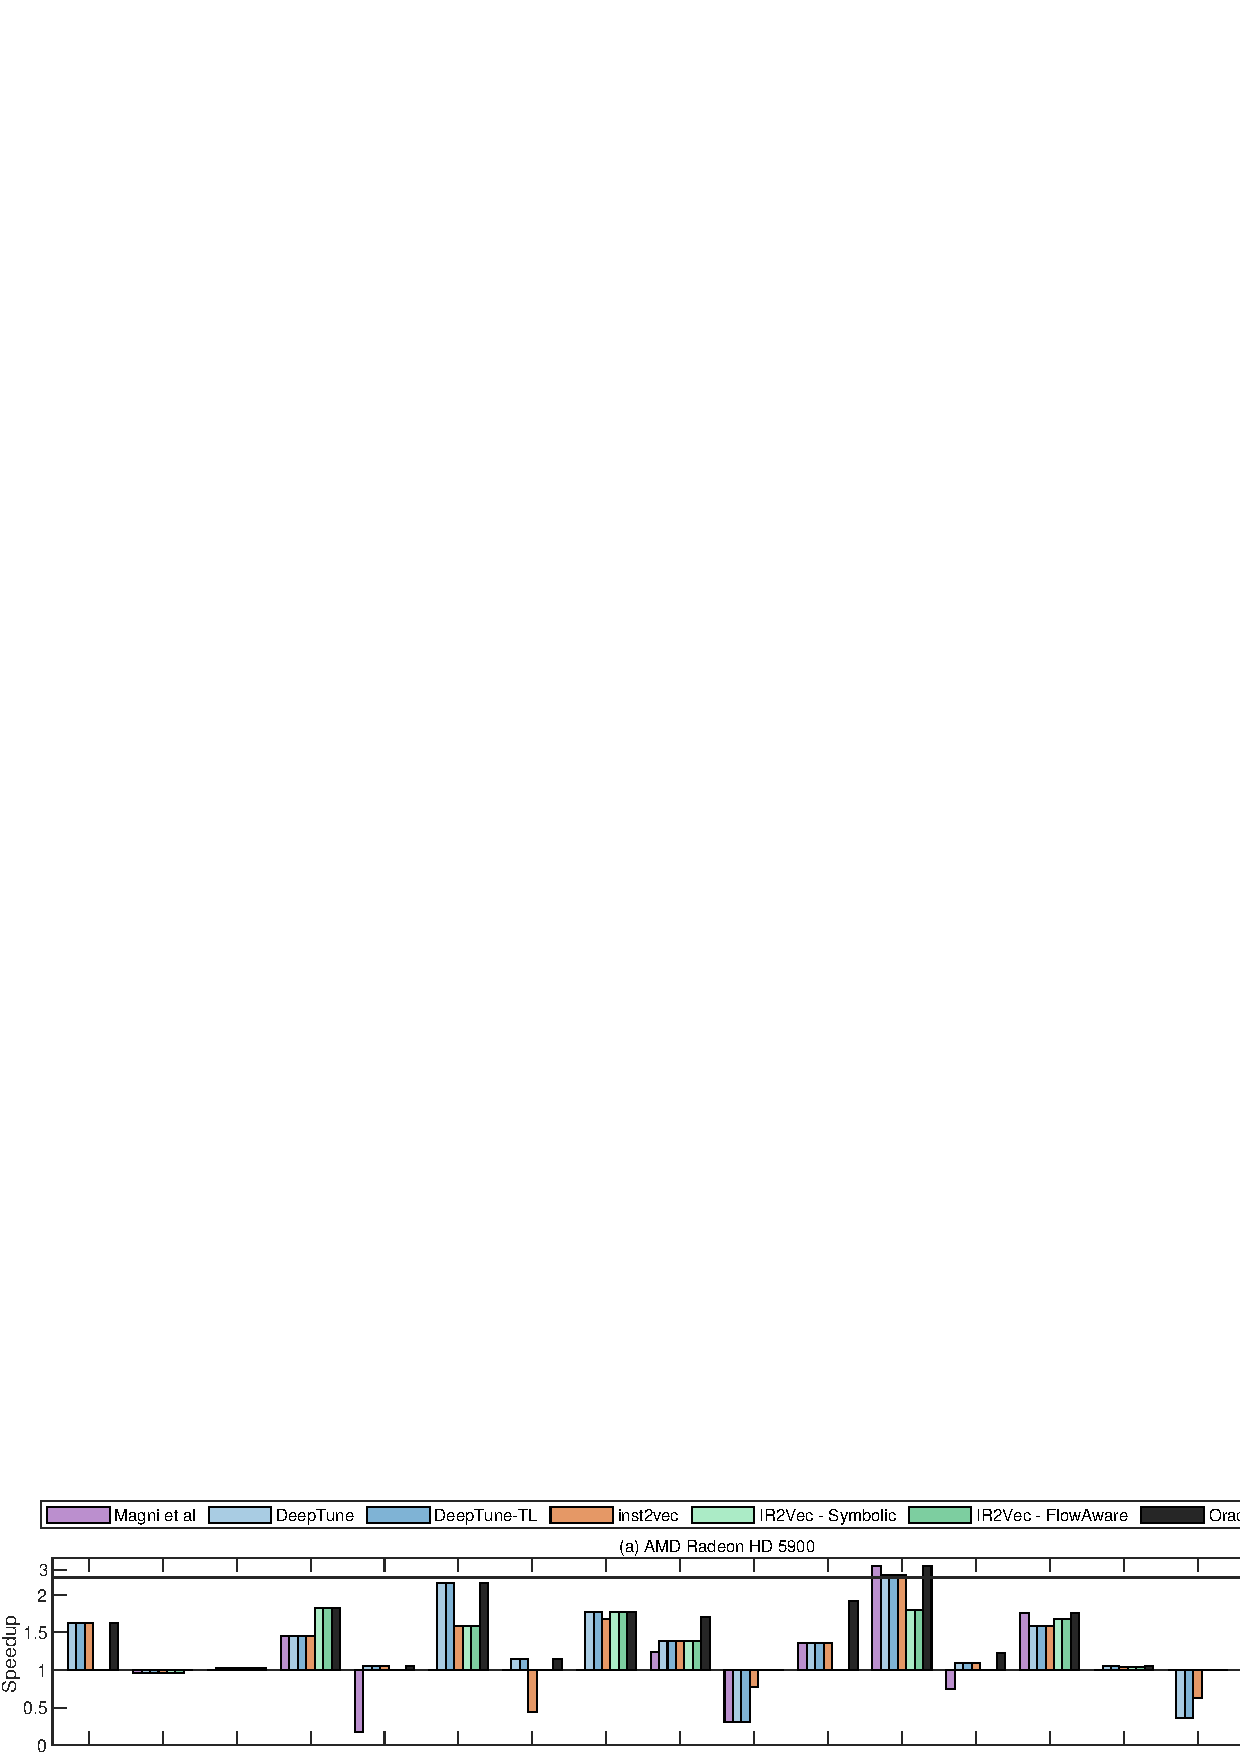
\includegraphics[scale=0.8, width=\textwidth]{figures/TC/new/radeon1-crop.pdf}
%     \end{tabular}
%     % \vspace{-5cm}
%     \begin{tabular}{@{}c@{}}
%         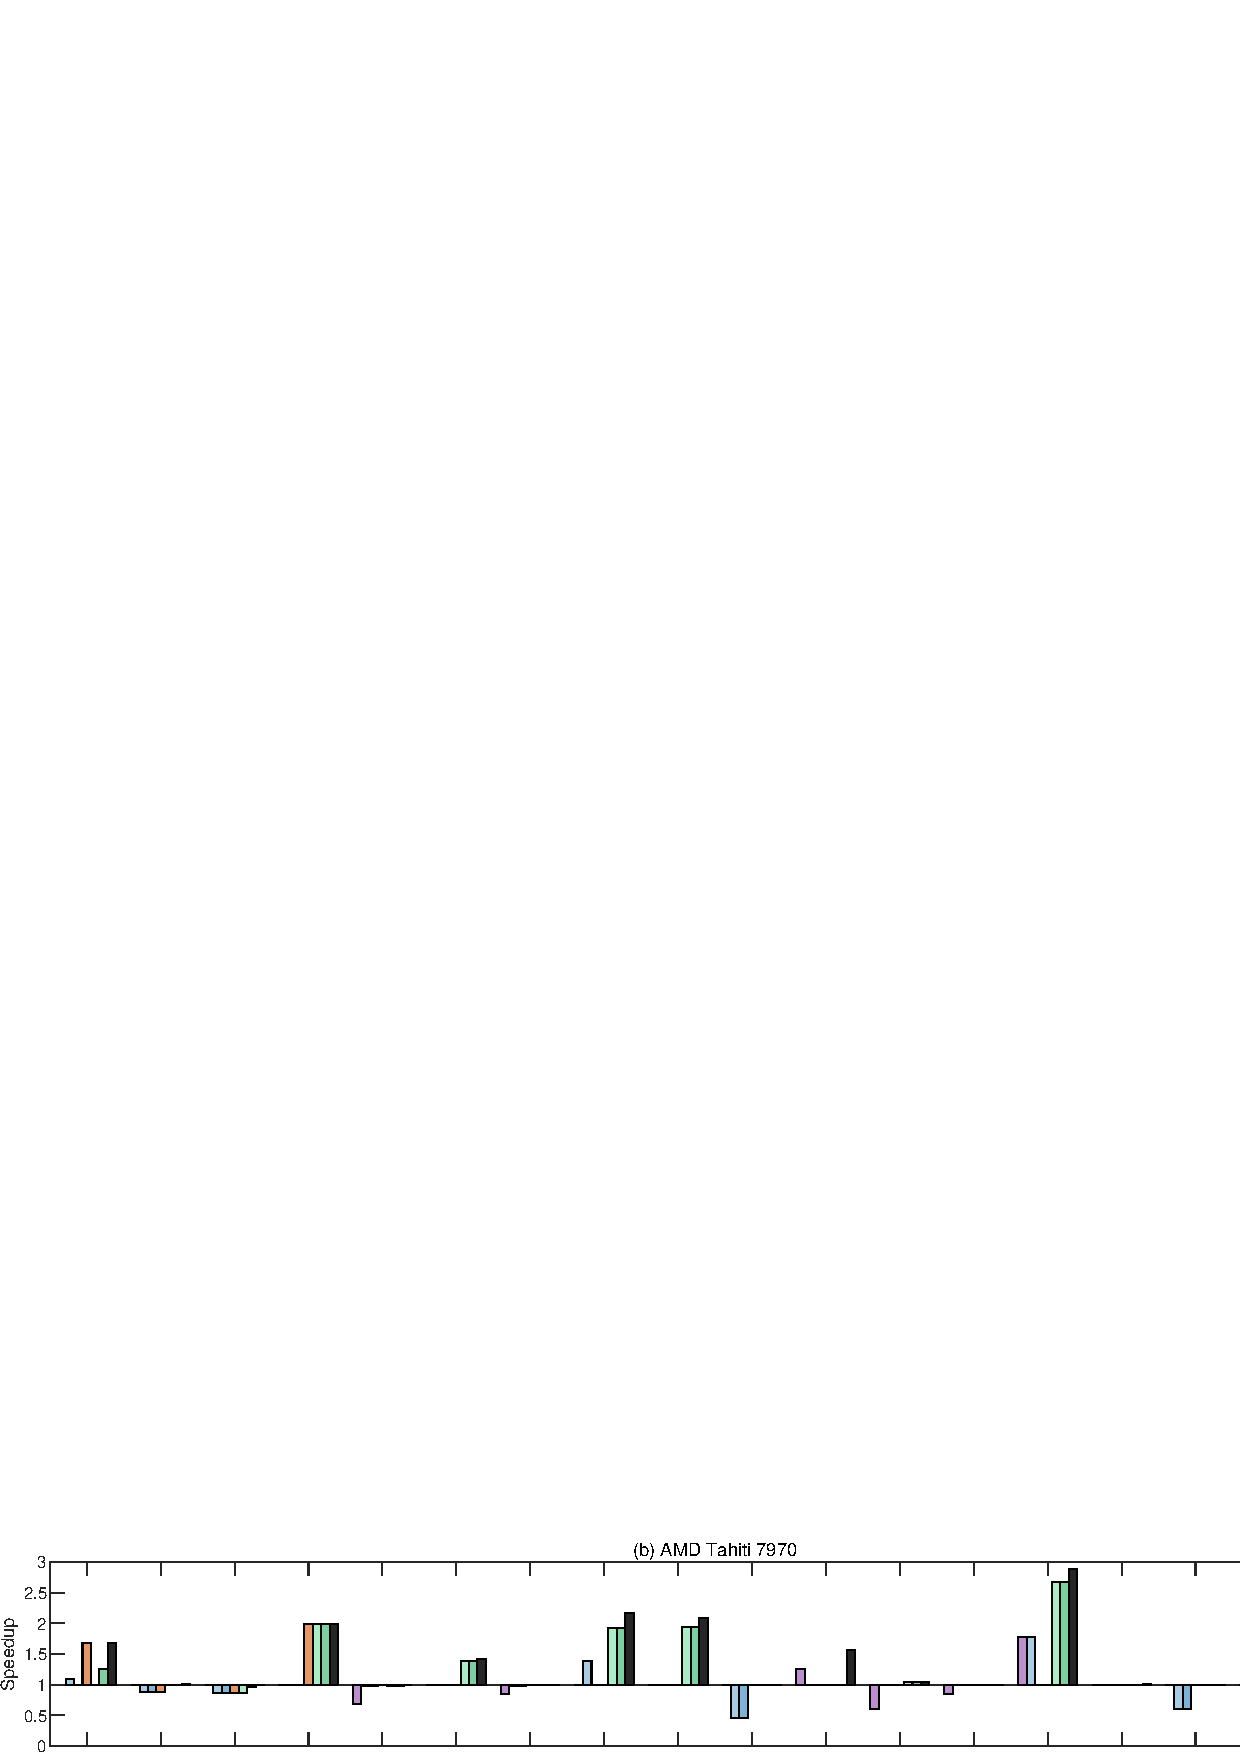
\includegraphics[scale=0.8, width=\textwidth]{figures/TC/new/tahiti2-crop.pdf}
%     \end{tabular}
%     \begin{tabular}{@{}c@{}}
%         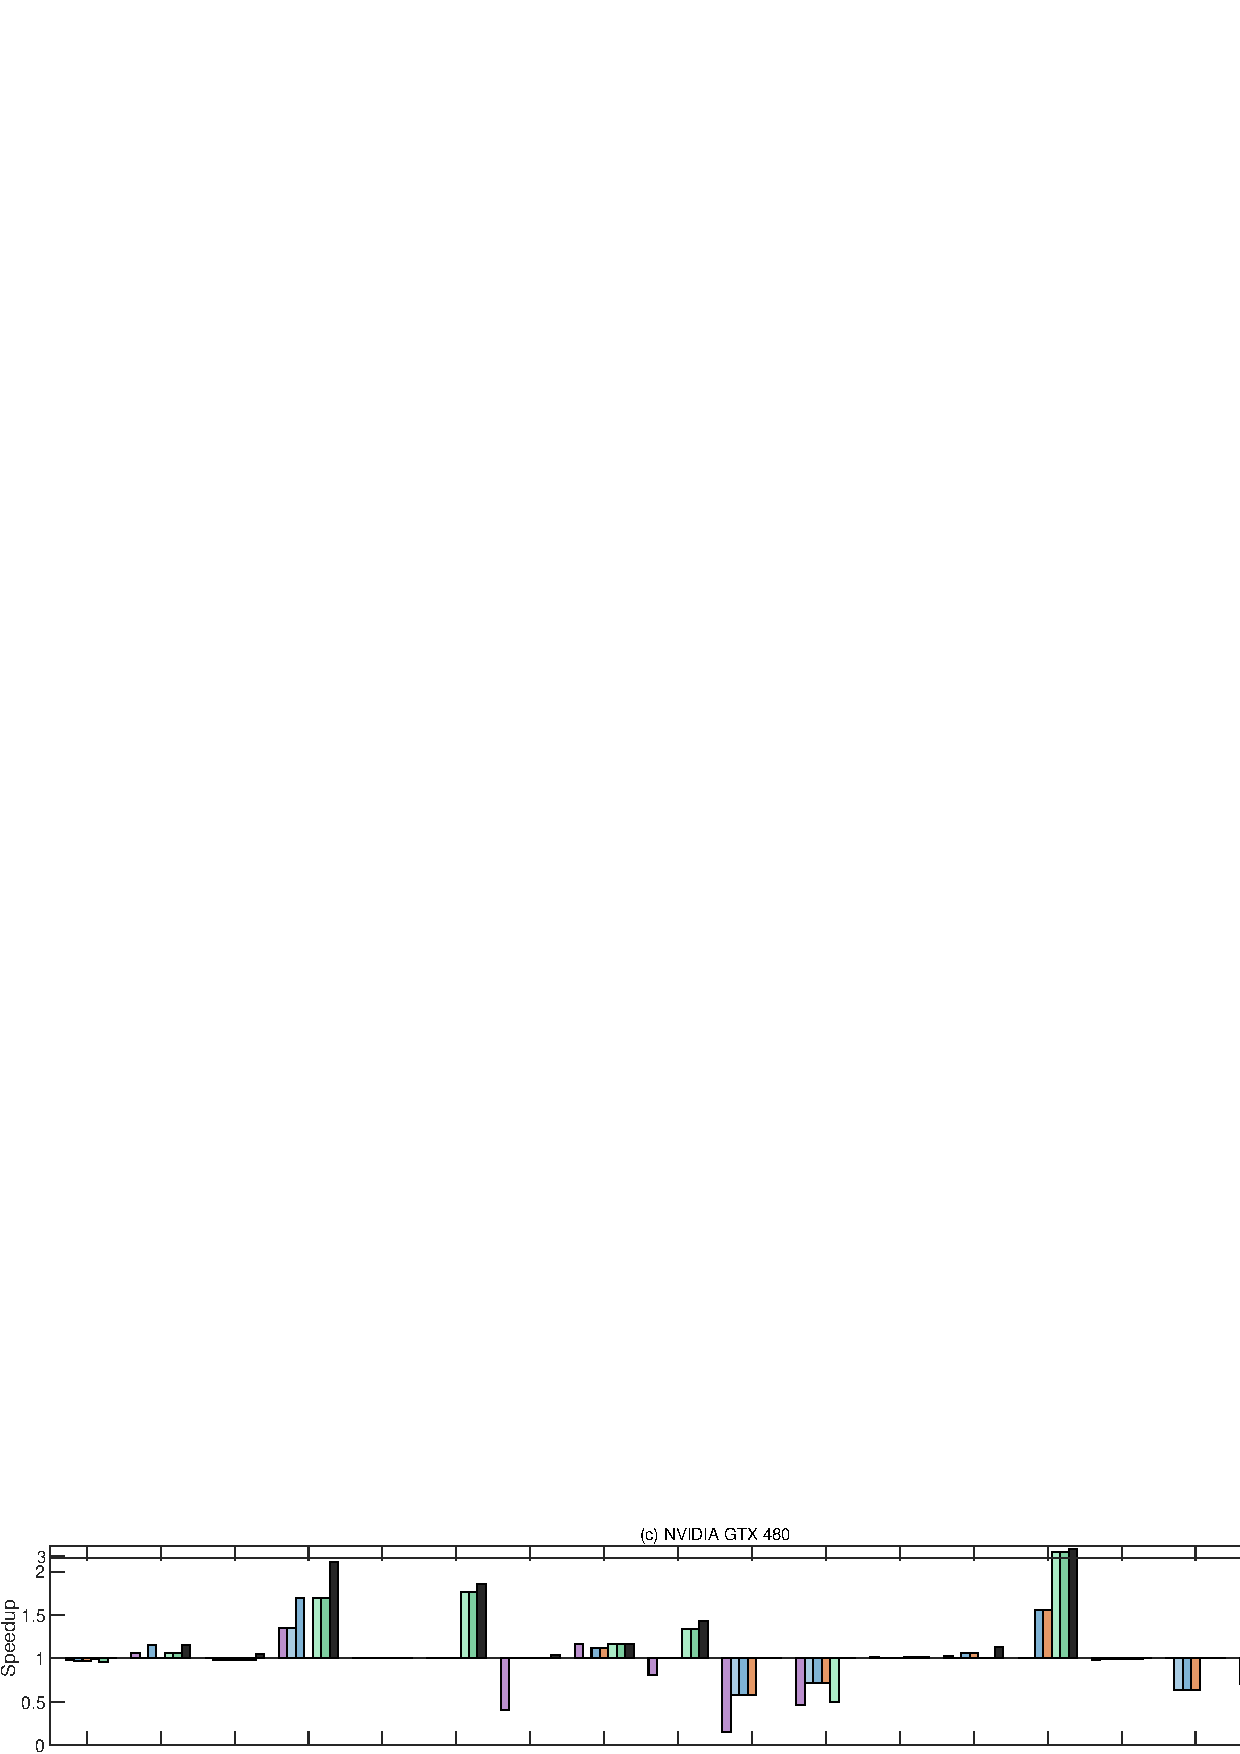
\includegraphics[scale=0.8, width=\textwidth]{figures/TC/new/gtx-crop.pdf}
%     \end{tabular}
%     \begin{tabular}{@{}c@{}}
%         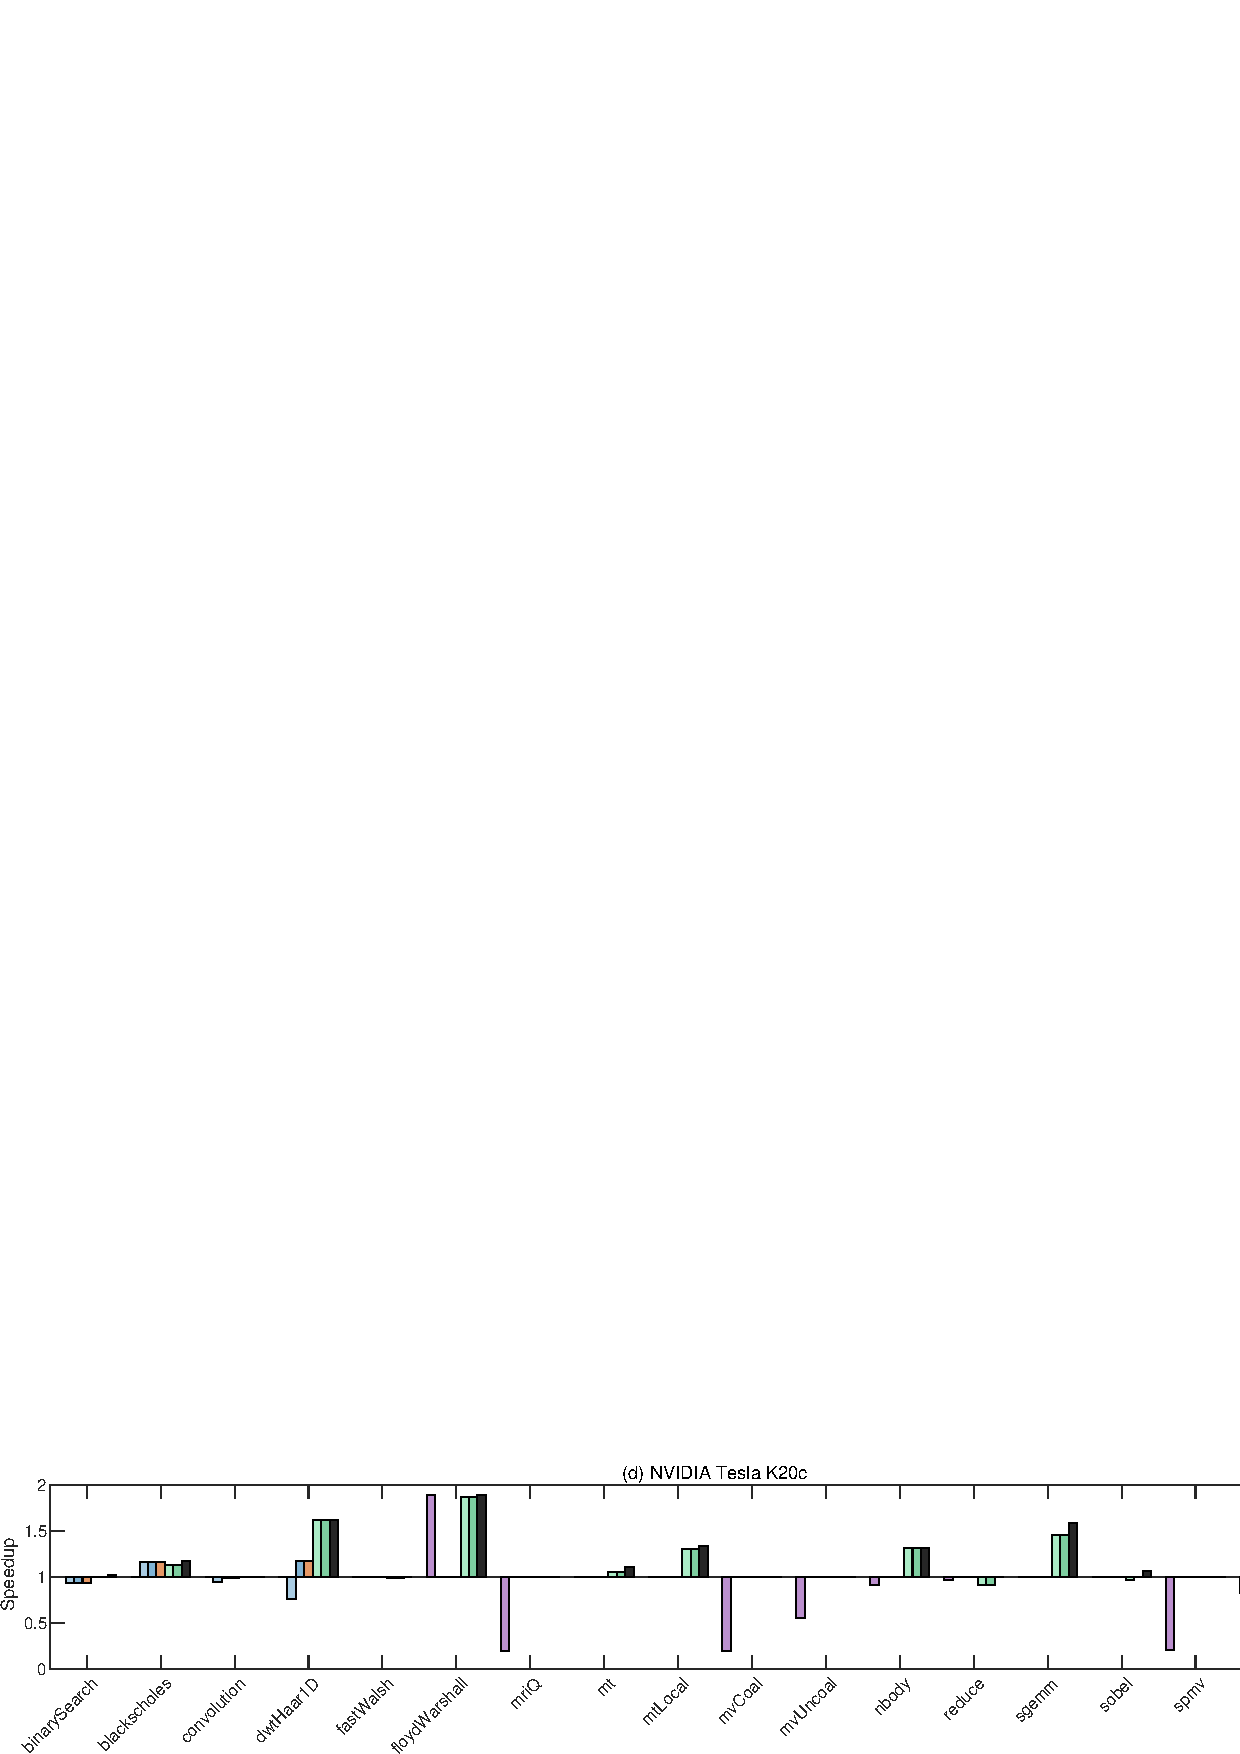
\includegraphics[scale=0.8, width=\textwidth]{figures/TC/new/tesla2-crop.pdf}
%     \end{tabular}
%     \caption{Plot showing the speedups achieved by predicted coarsening factors by various methods}
%     % \vspace*{-\baselineskip}
%     \label{fig:tcSpeedup}
%      \vspace*{-0.4cm}
% \end{figure}

\begin{figure}
    \centering
    \begin{tabular}{@{}c@{}}
        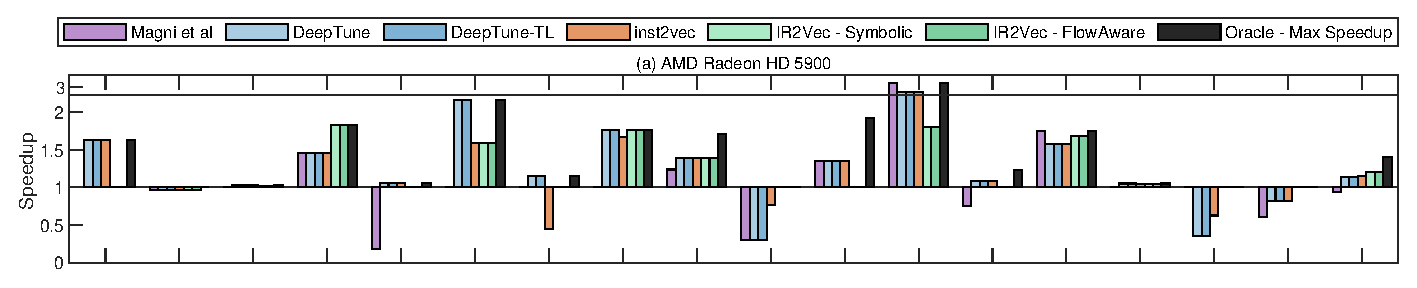
\includegraphics[scale=0.8, width=\textwidth]{figures/TC/radeon1-crop.eps}
    \end{tabular}
    % \vspace{-5cm}
    \begin{tabular}{@{}c@{}}
        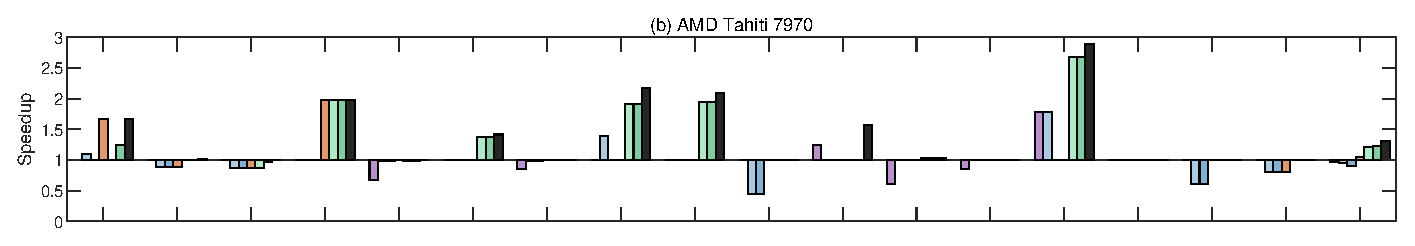
\includegraphics[scale=0.8, width=\textwidth]{figures/TC/tahiti2-crop.eps}
    \end{tabular}
    \begin{tabular}{@{}c@{}}
        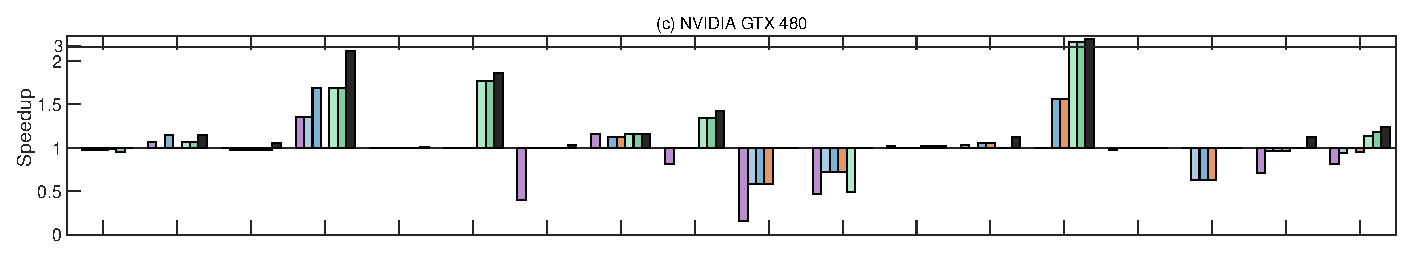
\includegraphics[scale=0.8, width=\textwidth]{figures/TC/gtx-crop.eps}
    \end{tabular}
    \begin{tabular}{@{}c@{}}
        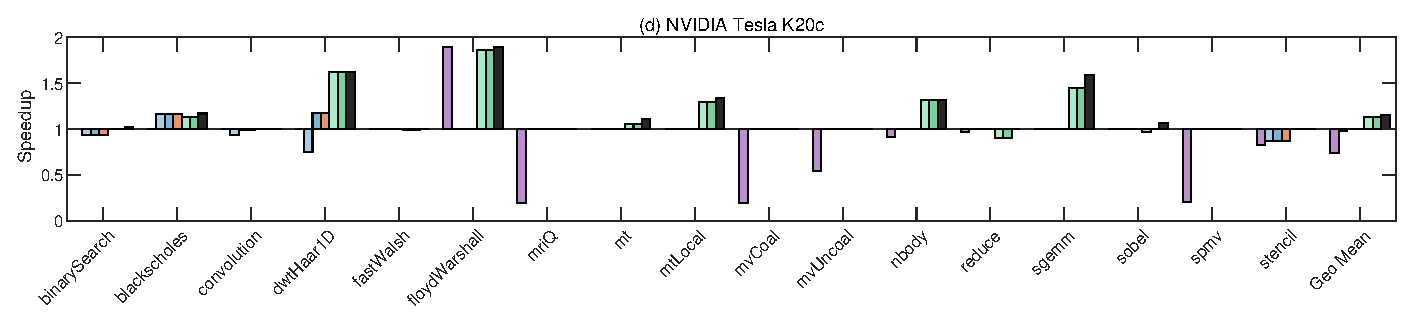
\includegraphics[scale=0.8, width=\textwidth]{figures/TC/tesla2-crop.eps}
    \end{tabular}
    \caption{Plot showing the speedups achieved by predicted coarsening factors by various methods}
    % \vspace*{-\baselineskip}
    \label{fig:tcSpeedup}
     \vspace*{-0.4cm}
\end{figure}


We are the \textit{first ones} to achieve a positive speedup on NVIDIA GTX 480; our \textit{Flow-Aware} and \textit{Symbolic} encodings obtain a speedup of $ 1.18\times$ and $ 1.13\times$ respectively when compared to $ 0.95\times$ and $ 0.99\times$ speedup achieved by inst2vec and DeepTune-TL. 
We get a speedup of $ 1.13\times$ with both of our proposed encodings on NVIDIA Tesla K20c. In contrast, DeepTune-TL and inst2vec obtain a speedup of $ 1.01\times$ on this platform.

On average, it can be seen that both encodings outperform the earlier methods for prediction of the thread coarsening factor on all the four platforms under consideration. 

\subsubsection{Slowdown}  Magni et al.~\cite{magni2014automatic} observe that \texttt{spmv} and \texttt{mvCoal} kernels have irregular dependences that causes a poor response to coarsening, and hence no performance improvement for them is possible.
For these kernels, IR2Vec obtains the baseline speedup \textit{without} resulting in a slowdown. In contrast, the earlier models result in negative speedups (Deeptune results in a slowdown upto $0.36$ $\times$ in AMD Radeon and inst2vec results in a slowdown of upto $0.63$ $\times$ in AMD Radeon and NVIDIA GTX). 
The same argument applies for \texttt{stencil} kernel (an iterative Jacobi stencil on 3D-grid), where the coarsening leads to slowdown (except in NVIDIA GTX), while IR2Vec still obtain the baseline speedup.

When compared to the other methods, we obtain the best speedup on about 70\% of the kernels on all platforms. 
It can be observed that the \textit{Flow-Aware} encodings \textit{rarely lead to slowdowns}; this happens in only 8/68 cases (17 benchmark-suits, across 4 platforms), even on these eight cases, the speedup is still close---within 10\%---of the baseline. 
Whereas, predictions by inst2vec and DeepTune-TL result in a slowdown in 18 and 21 cases.
We believe that this is because of the flow information associated with the obtained vectors.

\paragraph{Training}
Our model takes lesser time of $\approx$10 seconds for training when compared to $\approx$11 hours of training time needed by DeepTune-TL and $\approx$1 hour of training time needed (and 77K and 69K parameters used) by DeepTune and NCC approaches. 
This results in $\approx 360\times$--$3960\times$ reduction of training time, and again, achieving good speedups. 


\section{Conclusion}\label{sec:tc:conclusion}
We are able to achieve better results with respect to the prior work in term of both accuracy. Additionaly, the training time of the model is far better then the others.